\subsubsection{Limitation}

Prediction cost in baseline method consists of following two parts.

\begin{enumerate}
	\item Search cost for the cell which contains the key. This cost will be equal to $log_{2}N_{1}$, where $N_{1}$ is the number of cells into which mapped values are divided.
	
	\item Cost associated with sequentially comparing the query point key value against keys inside the cell found in previous search. On average this cost will be equal to $N_{2}\div2$, where $N_{2}$ is the number of keys in a cell.   
	
If cell size is large, number of cells will be smaller, number of keys per cell will be higher, resulting in higher cost of sequential scan with in the cell. 
\end{enumerate}
Consider the example in figure \ref{fig:BaseLine_Method_Limitation}. Dataset is divided into 3 sections based on the mapped values. Any point or range query in the second triangle(page) will result into a sequential scan through all 9 keys in the cells.

\begin{figure*}[t]
    \centering
    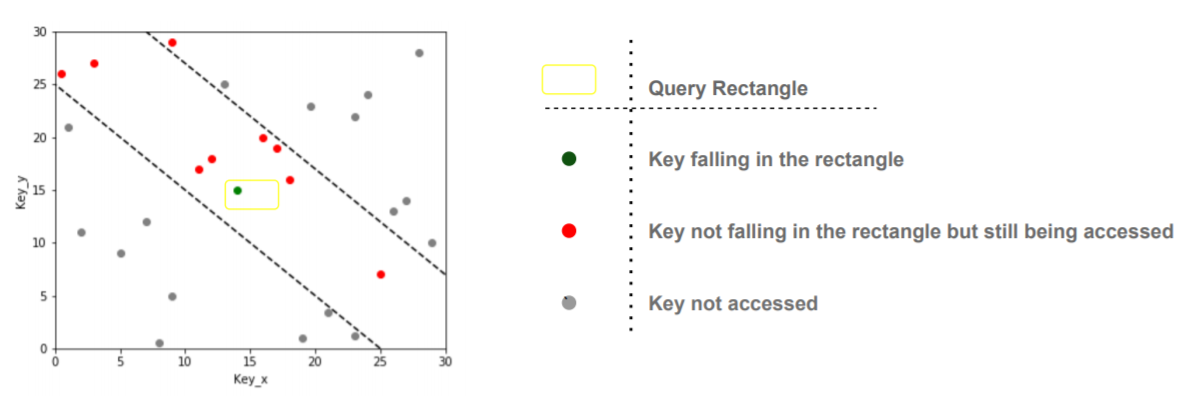
\includegraphics[width=1\textwidth]{graphs/Lisa_Baseline_Model_Limitation.png}
    \caption{Baseline Method Limitation }
    \label{fig:BaseLine_Method_Limitation}
\end{figure*}



\subsubsection {Lisa Baseline model search optimization}
%In lisa baseline model, we need to linearly search for the query key in a cell. 
In case of high dimensional key values, key with in a page can not be searched with mapped value, as a large number of keys can have the same mapped value. However for the 2 dimensional scenario, we can get considerable savings in search cost by replacing sequential scan based on keys values to binary search based on mapped value. Once mapped value is found using binary search, we do a look up in its neighbourhood based on 2 dimensional key value. As shown in table \ref{baselinesearch_optimization}, we get significant savings in the query time with this approach.

\begin{table}[ht]
	\centering
	\begin{tabular}{||p{0.15\textwidth}<{\centering}|p{0.2\textwidth}<{\centering}| p{0.1\textwidth}<{\centering}|p{0.15\textwidth}<{\centering}|p{0.15\textwidth}<{\centering}|p{0.15\textwidth}<{\centering}||}
		\hline
		Training/Test Data Size& Model & No. of cells & Build Time(ms) & Avg Query Time(ms) & Memory Size(KB)\\ [0.5ex] 
		\hline
		\hline
		10,000& Lisa Baseline & 10 & 11.1208 & 0.284191 & 313.77\\
		\hline
		10,000& Lisa Baseline & 100 & 12.0108 & 0.277918 & 315.85\\
		\hline
		10,000& Lisa Baseline & 1000 & 12.7589 & 0.276572 & 336.97\\
		\hline
		\hline
	\end{tabular}
	\label{baseline_search_optimization}
	\caption{Experimental results for baseline model with search optimization, Training Data Size : 10,000 points}
\end{table}

\begin{table}[ht]
	\centering
	\begin{tabular}{||p{0.15\textwidth}<{\centering}|p{0.2\textwidth}<{\centering}| p{0.1\textwidth}<{\centering}|p{0.15\textwidth}<{\centering}|p{0.15\textwidth}<{\centering}|p{0.15\textwidth}<{\centering}||}
		\hline
		Training/Test Data Size& Model & No. of cells & Build Time(ms) & Avg Query Time(ms) & Memory Size(KB)\\ [0.5ex] 
		\hline
		\hline
		100,000& Lisa Baseline & 10 & 112.973 & 0.285525 & 313.77\\
		\hline
		100,000& Lisa Baseline & 100 & 114.318 & 0.282053 & 315.85\\
		\hline
		100,000& Lisa Baseline & 1000 & 116.699 & 0.280637 & 336.97\\
		\hline
		\hline
	\end{tabular}
	\label{baseline_search_optimization}
	\caption{Experimental results for baseline model with search optimization, Training Data Size : 100,000 points}
\end{table}

\begin{table}[ht]
	\centering
	\begin{tabular}{||p{0.15\textwidth}<{\centering}|p{0.2\textwidth}<{\centering}| p{0.1\textwidth}<{\centering}|p{0.15\textwidth}<{\centering}|p{0.15\textwidth}<{\centering}|p{0.15\textwidth}<{\centering}||}
		\hline
		Training/Test Data Size& Model & No. of cells & Build Time(ms) & Avg Query Time(ms) & Memory Size(KB)\\ [0.5ex] 
		\hline
		\hline
		1,000,000& Lisa Baseline & 10 & 1116.51 & 0.240508 & 313.77\\
		\hline
		1,000,000& Lisa Baseline & 100 & 1118.85 &0.235858 & 315.85\\
		\hline
		1,000,000& Lisa Baseline & 1000 & 1134.88 & 0.234435 & 336.97\\
		\hline
		\hline
	\end{tabular}
	\label{baseline_search_optimization}
	\caption{Experimental results for baseline model with search optimization, Training Data Size : 1,000,000 points}
\end{table}

\comm{
\begin{table}
	\centering
	\begin{tabular}{||p{0.15\textwidth}<{\centering}|p{0.2\textwidth}<{\centering}| p{0.1\textwidth}<{\centering}|p{0.15\textwidth}<{\centering}|p{0.15\textwidth}<{\centering}|p{0.15\textwidth}<{\centering}||}
		\hline
		Training/Test Data Size& Model & No. of cells & Build Time(s) & Avg Query Time(s) & Memory Size(KB)\\ [0.5ex] 
		\hline
		\hline
		10,000& Lisa Baseline & 10 & 0.034 & 0.0005 & 313.77\\
		\hline
		10,000& Lisa Baseline & 100 & 0.023 & 0.0005 & 315.85\\
		\hline
		10,000& Lisa Baseline & 1000 & 0.021 & 0.0005 & 336.97\\
		\hline
		100,000& Lisa Baseline & 10 & 0.175 & 0.0005 & 3126.2\\
		\hline
		100,000& Lisa Baseline & 100 & 0.167 & 0.0005 & 3128.3\\
		\hline
		100,000& Lisa Baseline & 1000 & 0.204 & 0.0005 & 3149.4\\
		\hline 
		1,000,000& Lisa Baseline & 10 & 1.559 & 0.0005 & 31251.3\\
		\hline
		1,000,000& Lisa Baseline & 100 &1.705 & 0.0005 & 31253.4\\
		\hline
		1,000,000& Lisa Baseline & 1000 & 2.002 & 0.0005 & 31274.5\\

		\hline
		\hline
	\end{tabular}
	\label{baseline_search_optimization}
	\caption{Experimental results for lisa baseline model with search optimization for small lognormal data}
\end{table}
}